%%%%%%%%%%%%%%%%%%%%%%%%%%%%%%%%%%%%%%%%%
% Wenneker Assignment
% LaTeX Template
% Version 2.0 (12/1/2019)
%
% This template originates from:
% http://www.LaTeXTemplates.com
%
% Authors:
% Vel (vel@LaTeXTemplates.com)
% Frits Wenneker
%
% License:
% CC BY-NC-SA 3.0 (http://creativecommons.org/licenses/by-nc-sa/3.0/)
% 
%%%%%%%%%%%%%%%%%%%%%%%%%%%%%%%%%%%%%%%%%

%----------------------------------------------------------------------------------------
%	PACKAGES AND OTHER DOCUMENT CONFIGURATIONS
%----------------------------------------------------------------------------------------

\documentclass[11pt]{scrartcl} % Font size
\usepackage{algorithmic}
%%%%%%%%%%%%%%%%%%%%%%%%%%%%%%%%%%%%%%%%%
% Wenneker Assignment
% Structure Specification File
% Version 2.0 (12/1/2019)
%
% This template originates from:
% http://www.LaTeXTemplates.com
%
% Authors:
% Vel (vel@LaTeXTemplates.com)
% Frits Wenneker
%
% License:
% CC BY-NC-SA 3.0 (http://creativecommons.org/licenses/by-nc-sa/3.0/)
% 
%%%%%%%%%%%%%%%%%%%%%%%%%%%%%%%%%%%%%%%%%

%----------------------------------------------------------------------------------------
%	PACKAGES AND OTHER DOCUMENT CONFIGURATIONS
%----------------------------------------------------------------------------------------

\usepackage{amsmath, amsfonts, amsthm} % Math packages

\usepackage{listings} % Code listings, with syntax highlighting

\usepackage[english]{babel} % English language hyphenation

\usepackage{graphicx} % Required for inserting images
\graphicspath{{Figures/}{./}} % Specifies where to look for included images (trailing slash required)

\usepackage{booktabs} % Required for better horizontal rules in tables

\numberwithin{equation}{section} % Number equations within sections (i.e. 1.1, 1.2, 2.1, 2.2 instead of 1, 2, 3, 4)
\numberwithin{figure}{section} % Number figures within sections (i.e. 1.1, 1.2, 2.1, 2.2 instead of 1, 2, 3, 4)
\numberwithin{table}{section} % Number tables within sections (i.e. 1.1, 1.2, 2.1, 2.2 instead of 1, 2, 3, 4)

\setlength\parindent{0pt} % Removes all indentation from paragraphs

\usepackage{enumitem} % Required for list customisation
\setlist{noitemsep} % No spacing between list items

%----------------------------------------------------------------------------------------
%	DOCUMENT MARGINS
%----------------------------------------------------------------------------------------

\usepackage{geometry} % Required for adjusting page dimensions and margins

\geometry{
	paper=a4paper, % Paper size, change to letterpaper for US letter size
	top=2.5cm, % Top margin
	bottom=3cm, % Bottom margin
	left=3cm, % Left margin
	right=3cm, % Right margin
	headheight=0.75cm, % Header height
	footskip=1.5cm, % Space from the bottom margin to the baseline of the footer
	headsep=0.75cm, % Space from the top margin to the baseline of the header
	%showframe, % Uncomment to show how the type block is set on the page
}

%----------------------------------------------------------------------------------------
%	FONTS
%----------------------------------------------------------------------------------------

\usepackage[utf8]{inputenc} % Required for inputting international characters
\usepackage[T1]{fontenc} % Use 8-bit encoding

\usepackage{fourier} % Use the Adobe Utopia font for the document

%----------------------------------------------------------------------------------------
%	SECTION TITLES
%----------------------------------------------------------------------------------------

\usepackage{sectsty} % Allows customising section commands

\sectionfont{\vspace{6pt}\centering\normalfont\scshape} % \section{} styling
\subsectionfont{\normalfont\bfseries} % \subsection{} styling
\subsubsectionfont{\normalfont\itshape} % \subsubsection{} styling
\paragraphfont{\normalfont\scshape} % \paragraph{} styling

%----------------------------------------------------------------------------------------
%	HEADERS AND FOOTERS
%----------------------------------------------------------------------------------------

\usepackage{scrlayer-scrpage} % Required for customising headers and footers

\ohead*{} % Right header
\ihead*{} % Left header
\chead*{} % Centre header

\ofoot*{} % Right footer
\ifoot*{} % Left footer
\cfoot*{\pagemark} % Centre footer
 % Include the file specifying the document structure and custom commands
%\usepackage[demo]{graphicx}
%\usepackage{caption}
\usepackage{subcaption}
\usepackage{float}
\usepackage{listings}
\usepackage[showframe=true]{geometry}
\usepackage{changepage}

%----------------------------------------------------------------------------------------
%	TITLE SECTION
%----------------------------------------------------------------------------------------

\title{	
	\normalfont\normalsize
	\textsc{Università degli Studi di Trieste}\\ % Your university, school and/or department name(s)
	\vspace{25pt} % Whitespace
	\rule{\linewidth}{0.5pt}\\ % Thin top horizontal rule
	\vspace{20pt} % Whitespace
	{\huge First FHPC Assignment}\\ % The assignment title
	\vspace{12pt} % Whitespace
	\rule{\linewidth}{2pt}\\ % Thick bottom horizontal rule
	\vspace{12pt} % Whitespace
}

\author{\LARGE Nicola Domenis} % Your name

\date{\normalsize\today} % Today's date (\today) or a custom date

\begin{document}

\maketitle % Print the title

%----------------------------------------------------------------------------------------
%	FIGURE EXAMPLE
%----------------------------------------------------------------------------------------

\section{Preview}
 
In this assignment we will present the following subjects:

\begin{itemize}
	\item the analysis of the computational power of our laptop and smartphone;
	\item the analysis of a strong scaling model for a simple addition problem;
	\item the resolution of a scalability problem for a simple parallel code that computes pi;
	\item the parallel implementation of the above addition program;
	\item the scalability of the addition program.
\end{itemize}


%------------------------------------------------
\section{section 0}
\subsection{Laptop theoretical peak performance}

We want to calculate the theoretical peak performance of our own portable computer by using the formula \textit{theoretical peak performance} = clock frequency x FLOPs x number of cores.
We gather that \textit{clock frequency} $= 2.90 Ghz$,$ FLOPs = 16$ and \textit{number of cores} $= 2$ for our computer architecture,an intel i7 with a Kaby Lake microarchitecture; thus we compute \textit{theoretical peak performance} $= 92.8 GFlops/s$
%Vect_size = dimensione di registro vettoriale stessa operaaxione nello stesso momento diviso dimensione double:andiamo a vedere se ci sono le sigle (mmx sse)128bit 2 double (avx avx2) 256bit 4 double (avx512)512bit 8 double
%primo fattore
%
%cercare FMA fused multiply addiction A = BxC+D  vec
%vector_size*2*#fma

%quanti cicli ci vogliono? pensiamo che sia 1 = 1*vector_size*2*#fma

%numero di operazioni in double precision
%\begin{figure}
%\begin{adjustwidth}{-2cm}{}
\begin{table}[H]
		\begin{tabular}[H]{l| l| l| l| l| l }
			&Your model&CPU&Frequency&Number of Cores&Peak Performance\\
			laptop& Asus F556U & Intel Core i7-7500 &$2.90$ GHz&2&92.8 GFLOPs/s
		\end{tabular}
	\label{Result}
\end{table}
%\end{adjustwidth}
%\end{figure}

\subsection{Smartphone theoretical peak performance}
We installed "`Mobile Linpack"' app and we run a few test. We report here some results,even on repeated trials: 
%\begin{figure}
\begin{adjustwidth}{-2cm}{}
	\begin{tabular}[H]{l| p{0.2\textwidth}| l |l| l|l }
		\hline
			&Model& Sustained performance&Matrix size&Peak performance&Memory\\
			\hline
			Cellphone&Samsung Galaxy XCover 4 &114,81 Mflops/s &250 &not calculated&16,00 GB\\
			& &145.53 Mflop/s&500& &\\
			& &157.5 Mflop/s&800& &\\
			& &201.32 Mflop/s&800& &\\
			& &155.93 Mflop/s&900& &\\
			& &109.88 Mflop/s&1000& &\\
			& &103.14 Mflop/s&2000& &\\
		\end{tabular}
\end{adjustwidth}
%\end{figure}

\subsection{Laptops,smartphones and the top 500}
Let's check now whether our technologies would have competed with the Top500 supercomputers in the past:
%\begin{figure}
\begin{adjustwidth}{-2cm}{}
	\begin{tabular}[H]{p{0.15\textwidth}| p{0.15\textwidth}| p{0.15\textwidth} | p{0.3\textwidth}| p{0.3\textwidth}}
		\hline
			&Model&Performance&Top 500 year\& position&number 1 HPC system\\
			\hline
			Smartphone&Samsung Galaxy XCover 4 &201,32 Mflops/s &does not enter in the top500 of the first year of measurement, the 500th Supercomputer has an Rmax of 0.5 GFlops/s (equal to 2.4 times our smartphone peak performance)& Numerical Wind Tunnel,Fujitsu National Aerospace Laboratory of Japan is first in the year 1993 with a Rmax equal to 124.0 GFlops/s (equal to 616 times our cellphone's sustained peak performance)\\
			\hline
			Laptop&ASUS F556U&92.8 GFLOPs/s& 3rd position at nov 1993. Remains in the top 10 until nov 1996 & We have the same top position with a Rpeak equal to 235.8 GFlops/s(equal to 2.5 times our laptop's theoretical peak performance)\\
		\end{tabular}
\end{adjustwidth}
%\end{figure}

%\begin{table}
	%\centering
		%\begin{tabular}{l| l| l |l| l| l}
			%&Model& Sustained performance&Matrix size&Peak performance&Memory\\
			%Cellphone&Samsung Galaxy XCover 4 &114,81 Mflops/s &250 &not calculated&16,00 GB
			%&&145.53 Mflop/s&500&&
			%&&157.5 Mflop/s&800&&
			%&&109.88 Mflop/s&1000&&
		%\end{tabular}
	%\label{Quick test parameters and results}
%\end{table}

%----------------------------------------------------------------------------------------
%	TEXT EXAMPLE
%----------------------------------------------------------------------------------------

\section{Section 1}

\subsection{Model for a serial and parallel summation of n numbers}
Here we discuss about modeling a simple program which consists of summing n numbers.
A simple pseudocode for the serial program would be:


\begin{algorithmic}

\STATE {Data:array $A[]$ of values}
\FOR{i from 1 to n} \STATE {sum = sum + A[i]} \ENDFOR
\RETURN{sum}
\end{algorithmic}

If we choose $T_{comp}$ as the time to compute a floating point operation we could calculate the total time of a serial computation as
$T_s = N * T_{comp}$,whereas the code simply computes N times(the size of the problem) the sum of two values.

For the parallel program we complicate a little the execution:

\begin{algorithmic}

\STATE {Data:array $A[]$ of values}
\STATE {Environment: p parallel processors}
\IF {Master process}

		\STATE{Read and Split $A[]$ into p subarrays $A_i[]$}
		\STATE{Send $p-1$ subarrays to the other $p-1$ processors}
		\FOR{i from $1$ to n/p} \STATE {$sum_0 = sum_0 + A_0[i]$} \ENDFOR
		\STATE{Collect the resulting $p-1$ values $sum_i$ from the processors}
		\FOR{i from $1$ to p} \STATE {$sum = sum + sum_i$} \ENDFOR
\ENDIF
\IF {Slave process}
	\STATE{Receive subarrays $A_i[]$ from the Master process}
	\FOR{i from 1 to n/p} \STATE {$sum_i = sum_i + A_i[i]$} \ENDFOR
	\STATE{Send $sum_i$ back to the Master process}
\ENDIF
\RETURN{sum}
\end{algorithmic}

If we define the times $T_{read}$ to indicate the time needed to read a variable,and $T_{comm}$ to indicate the time needed to communicate a variable, we can deduce the theoretical execution time of the model:
\  
\begin{algorithmic}
		\STATE{Read and Split $A[]$ into p subarrays $A_i[]$}
		\STATE{EXECUTION TIME: $T_{read}$}
\end{algorithmic}
\ 
\begin{algorithmic}
		\STATE{Send $p-1$ subarrays to the other $p-1$ processors}
		\STATE{EXECUTION TIME: $T_{comm}*(p-1)$}
\end{algorithmic}
\ 

\begin{algorithmic}

\FOR{i from $1$ to $n/p$} \STATE {$sum_i = sum_i + A_i[i]$} \ENDFOR
\STATE{EXECUTION TIME: $n/p * T_{comp}$}
\STATE{This is a parallel execution, the subarrays are added inside each processor}	
\end{algorithmic}

\ 
\begin{algorithmic}
\STATE{Send $sum_i$ back to the Master process}
\STATE{EXECUTION TIME: $(p-1)*T_{comm}$}
\end{algorithmic}
\ 
\begin{algorithmic}
		\FOR{i from $1$ to p} \STATE {$sum = sum + sum_i$} \ENDFOR
		\STATE{EXECUTION TIME: $(p-1)*T_{comp}$}
\end{algorithmic}

The total sum of the execution times gives $T_p = T_{read} + (p-1+n/p)*T_{comp}+2*T_{comm}(p-1)$. We can calculate it with the theoretical values $T_{comp} =2 \times 10^{-9}$,$T_{read}= 1 \times 10^{-4}$ and $T_{comm}= 1 \times 10^{-6}$
%----------------------------------------------

\subsection{Scalability of the Model}

Once we have the theoretical $T_p$ and $T_s$ we can calculate the Speedup given by the formula $Speedup(p)=T_s/T_p$ . We give the following plots on the variable $p$:

%\begin{figure}
%\centering
%\begin{subfigure}{.5\textwidth}
	%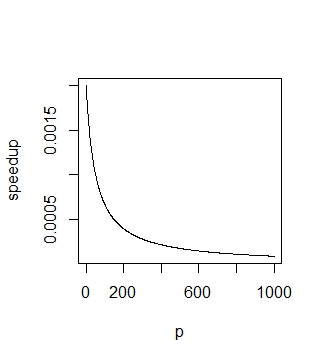
\includegraphics[width=0.5\columnwidth]{Rplot_speedup_4} % Example image
	%\caption{Speedup for $N=10^2$,maximum: $speedup = 0.00199$ at $p = 1$}
%\end{subfigure}%
%\begin{subfigure}{.5\textwidth}
 %% [h] forces the figure to be output where it is defined in the code (it suppresses floating)
	%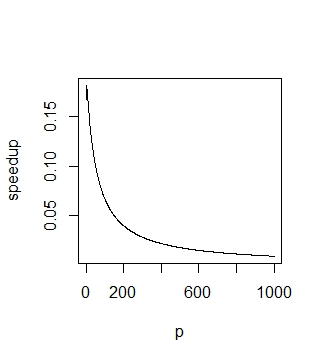
\includegraphics[width=0.5\columnwidth]{Rplot_speedup_3} % Example image
	%\caption{Speedup for $N=10^4$,maximum: $speedup = 0.180$ at $p = 3$}
 %\end{subfigure}
%\end{figure}

\begin{figure}[H] % [h] forces the figure to be output where it is defined in the code (it suppresses floating)
	\centering
	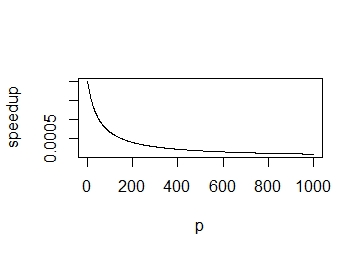
\includegraphics[width=0.6\columnwidth]{Rplot_speedup_sum_2} % Example image
	\caption{Speedup for $N=10^2$,maximum: $speedup = 0.002$ at $p = 1$}
\end{figure}


\begin{figure}[H] % [h] forces the figure to be output where it is defined in the code (it suppresses floating)
	\centering
	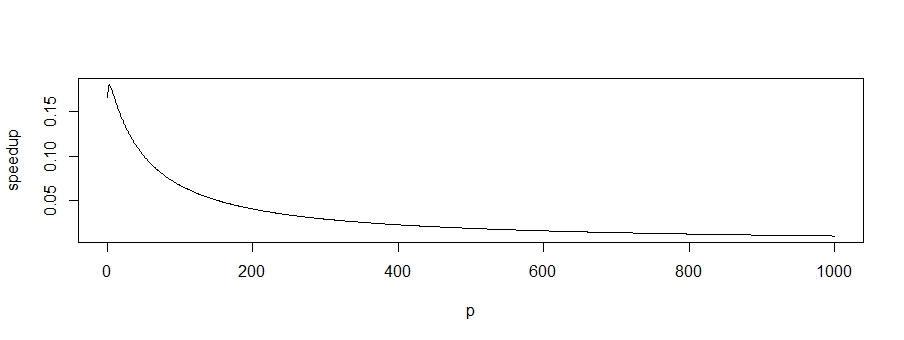
\includegraphics[width=0.6\columnwidth]{Rplot_speedup_sum_4} % Example image
	\caption{Speedup for $N=10^4$,maximum: $speedup = 0.181$ at $p = 3$}
\end{figure}
\begin{figure}[H] % [h] forces the figure to be output where it is defined in the code (it suppresses floating)
	\centering
	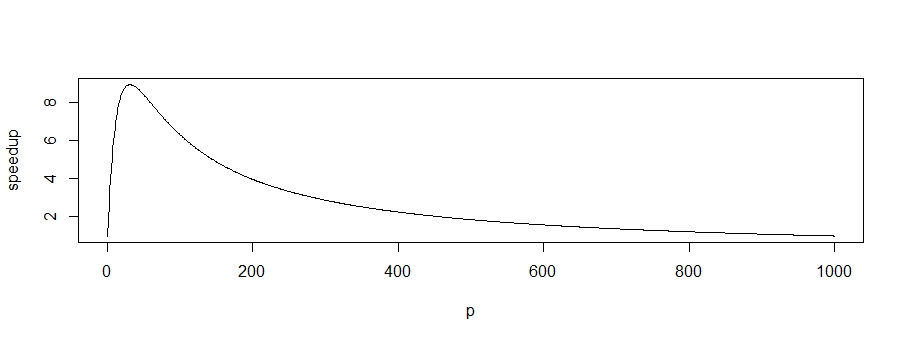
\includegraphics[width=0.6\columnwidth]{Rplot_speedup_sum_6} % Example image
	\caption{Speedup for $N=10^6$,maximum: $speedup = 8.91$ at $p = 32$}
\end{figure}
\begin{figure}[H] % [h] forces the figure to be output where it is defined in the code (it suppresses floating)
	\centering
	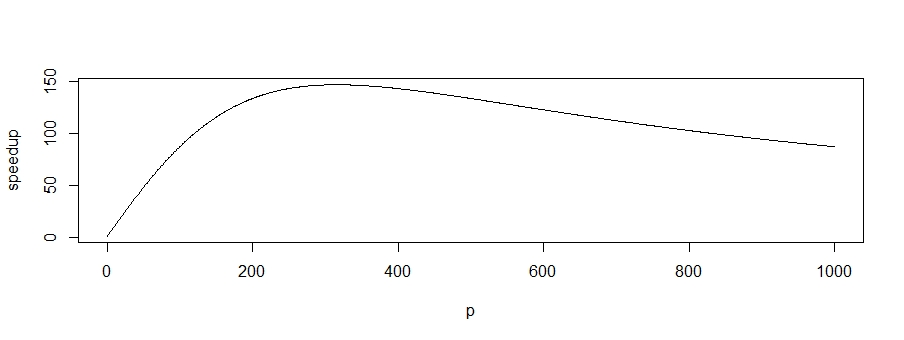
\includegraphics[width=0.6\columnwidth]{Rplot_speedup_sum_8} % Example image
	\caption{Speedup for $N=10^8$,maximum: $speedup = 147$ at $p = 316$}
\end{figure}
\begin{figure}[H] % [h] forces the figure to be output where it is defined in the code (it suppresses floating)
	\centering
	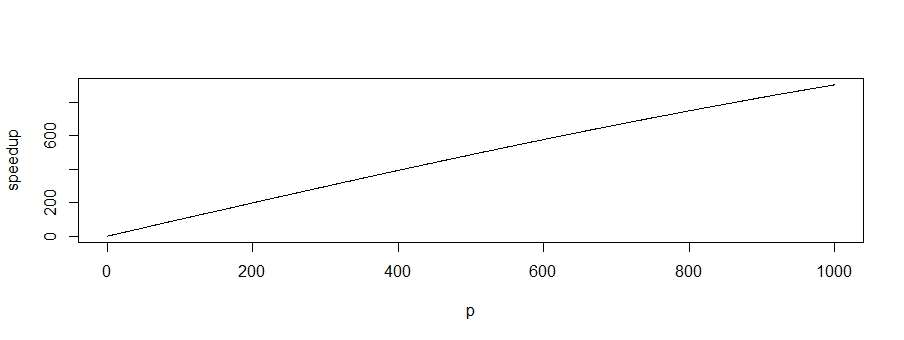
\includegraphics[width=0.6\columnwidth]{Rplot_speedup_sum_10} % Example image
	\caption{Speedup for $N=10^10$,maximum: $speedup = 905$ at $p = 1000$}
\end{figure}

We notice that as we increase N we get closer to a case of perfect scaling, on our number of processors. As N grows, adding a certain number of processors accelerates the calculations almost linearly.
If N is low,instead , we see that the problem starts scaling around $N=10^6$, where the speedup grows up to a maximum, and then decreases:the communication time overpowers the advantage of the parallelization, thus lowering the speedup.
 Simply adding processors to the calculus will not speed up the process because the time it takes to the master node to assign the subarrays to the slaves will grow as well.
The algorithm performs well if :
\begin{itemize}
	\item p corresponds to the maximum speedup;
	\item the maximum speedup is greater than 1: it makes the parallelization convenient.
\end{itemize}
%------------------------------------------------
\section{Section 2}

\subsection{\textit{mpi\_pi.c} and \textit{pi.c} execution}
We start by executing the two codes \textit{pi.c} and \textit{mpi\_pi.c} we have:

\begin{lstlisting}[language=bash]
  
$ g++ pi.c -o pi.x
$ time ./pi.x 10000000

 # of trials = 10000000 , estimate of pi is 3.141396400 

 # walltime : 0.19000000 

real    0m0.275s
user    0m0.271s
sys     0m0.001s
\end{lstlisting}
And the parallel file:
\begin{lstlisting}[language=bash]
$ mpicc mpi_pi.c -o mpi_pi.x
$ time mpirun -np 10 ./mpi_p.x 10000000

 # walltime on processor 1 : 0.02612305 

 # walltime on processor 2 : 0.03022003 

 # walltime on processor 3 : 0.02638388 

 # walltime on processor 4 : 0.03122497 

 # walltime on processor 5 : 0.02647901 

 # walltime on processor 6 : 0.02861810 

 # walltime on processor 7 : 0.03266811 

 # walltime on processor 8 : 0.02701306 

 # walltime on processor 9 : 0.03131413 

 # of trials = 10000000 , estimate of pi is 3.141720800 

 # walltime on master processor : 0.06575489 

real    0m1.890s
user    0m11.881s
sys     0m0.630s
\end{lstlisting}

We should get the longest time of all the parallel execution times of \textsc{mpi\_pi.x} in order to asses its speed.

Let's collect various run times for a different number of processors. 
%------------------------------------------------
\begin{adjustwidth}{2cm}{}
	\begin{tabular}[h]{l|l }
		\hline
			\# of processors&Maximum processor speed\\
			\hline
			1&0.19799113\\
			2&0.102010919\\
			4&0.0.05167317\\
			8&0.02782202\\
			16&0.01556611\\
			32&0.04725909\\
			64&0.04147911\\
		\end{tabular}
	\end{adjustwidth}
We notice that the serial execution time and the single processor parallel execution time differ because of the parallel overhead time: $usertime\_T_p(1)-usertime\_T_s+systime\_T_p(1)= 11.881-0.271+ 0.630= 12.24 s$ .This is the parallel overhead time for a single process.

Those values are plotted as:
\begin{figure}[H] % [h] forces the figure to be output where it is defined in the code (it suppresses floating)
	\centering
	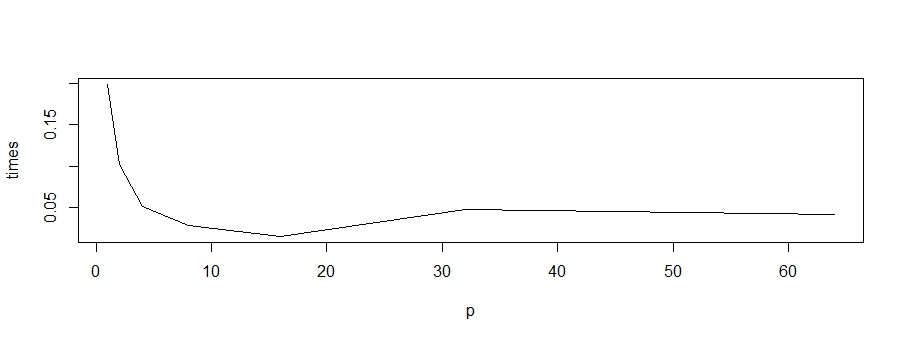
\includegraphics[width=0.6\columnwidth]{Rplot_pi_times_10millions} % Example image
	\caption{Execution time vs number of processors $N = 10^7$ }
\end{figure}

The time decreases inversely to the time. Now lets plot the speedup: 
\begin{figure}[H] % [h] forces the figure to be output where it is defined in the code (it suppresses floating)
	\centering
	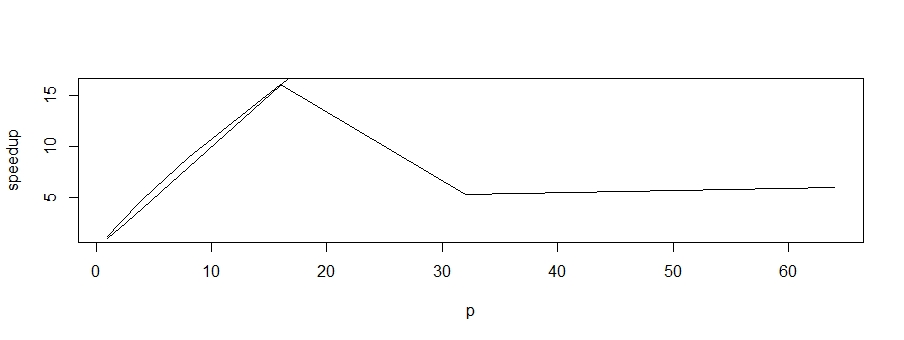
\includegraphics[width=0.6\columnwidth]{Rplot_pi_speedup_10millions} % Example image
	\caption{Speedup vs number of processors $N=10^7$}
\end{figure}
We see that it is not linear: the program scales only until around 20 processors.

Let's repeat our observations by having a larger problem size.
Here we have a plot that shows us the maximum execution time against the number of processors. Lets see the case$ N=10^8$
\begin{figure}[H] % [h] forces the figure to be output where it is defined in the code (it suppresses floating)
	\centering
	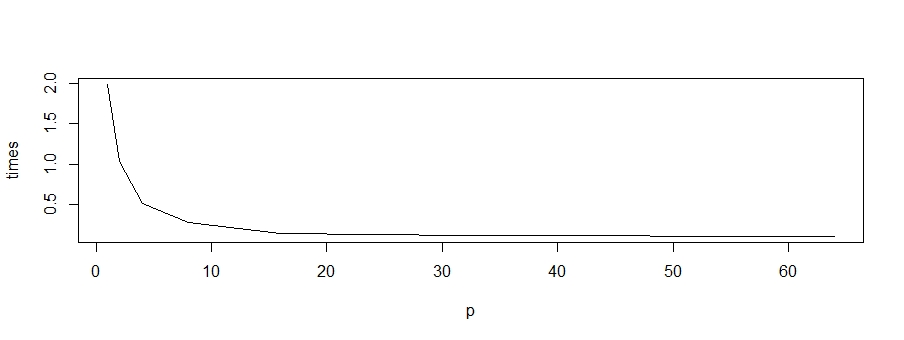
\includegraphics[width=0.6\columnwidth]{Rplot_pi_times_100millions} % Example image
	\caption{Execution time vs number of processors $N= 10^8$}
\end{figure}
We can see that the speedup  decreases for a large number of processors
\begin{figure}[H] % [h] forces the figure to be output where it is defined in the code (it suppresses floating)
	\centering
	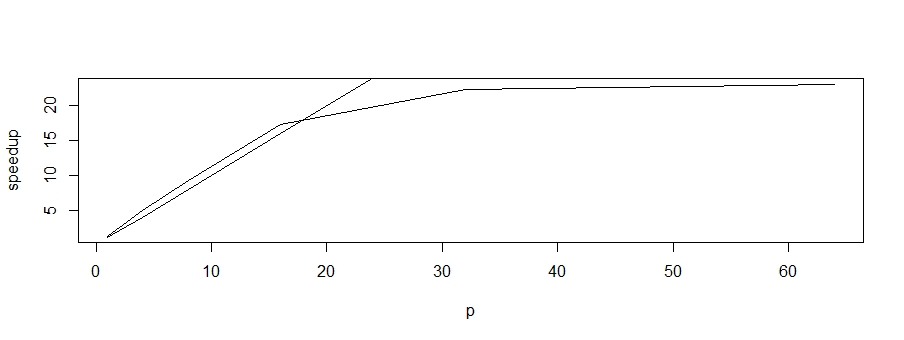
\includegraphics[width=0.6\columnwidth]{Rplot_pi_speedup_100millions} % Example image
	\caption{Speedup vs number of processors $N=10^8$}
\end{figure}
We can observe that the graph is rising closer to the drawn line, that represents the perfect speedup that is equal to p.
Lets see the same graphs for $N=10^9$:
\begin{figure}[H] % [h] forces the figure to be output where it is defined in the code (it suppresses floating)
	\centering
	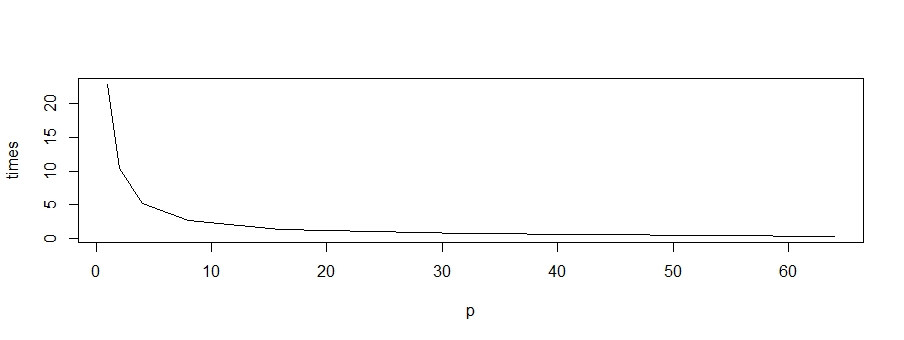
\includegraphics[width=0.6\columnwidth]{Rplot_pi_times_1billion} % Example image
	\caption{ Execution time vs number of processors $N= 10^8$}
\end{figure}
\begin{figure}[H] % [h] forces the figure to be output where it is defined in the code (it suppresses floating)
	\centering
	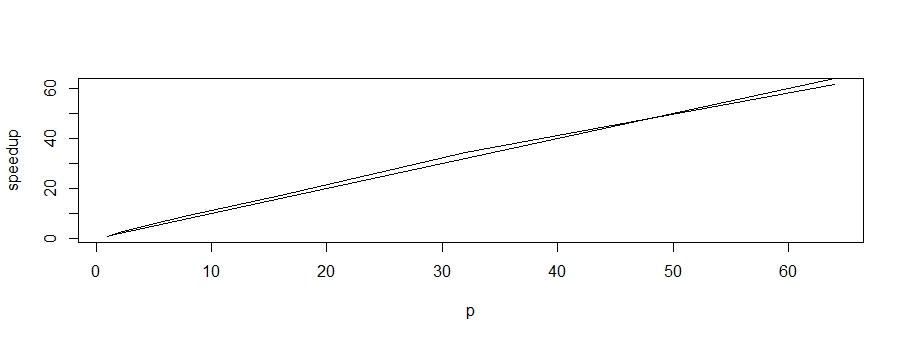
\includegraphics[width=0.6\columnwidth]{Rplot_pi_speedup_1billion} % Example image
	\caption{speedup vs number of processors $N= 10^9$}
\end{figure}

Here the speedup plot is linear, for 0<p<64, thus adding more processors increases linearly the execution time.
 We have analyzed the strong scalability of the model. 
\subsection{2.2 Parallel overhead}
Here we discuss about identifying a model for deducing the overhead of our program. We study the case where $N=10^7$ and we plot the difference between the maximum processor walltime
 and the minimum processor walltime for a different number of processors.
We obtain the following graph
\begin{figure}[H] % [h] forces the figure to be output where it is defined in the code (it suppresses floating)
	\centering
	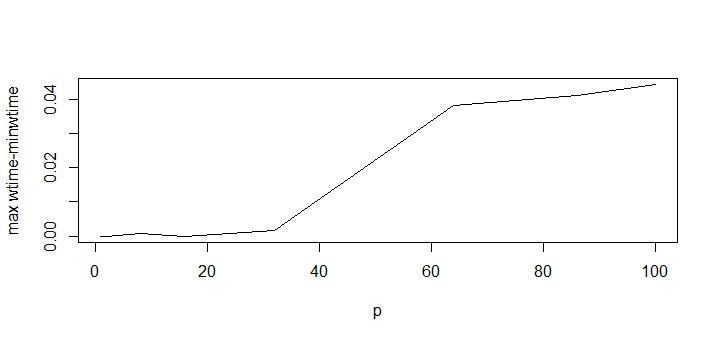
\includegraphics[width=0.6\columnwidth]{Rplot_pi_max_-_min} % Example image
	\caption{overhead vs number of processors $N= 10^9$}
\end{figure}

We can see that the overhead grows as p grows. This is explained by the fact that the overhead increases because of the accessory computation we adopt in order to manage more nodes.
\subsection{2.3 Weak scaling}

We run a shell script to automatically collect the runtimes for various proportional values of p and N. N is equal to $10^7*p$ as p grows.
We obtain the following plot
\begin{figure}[H] % [h] forces the figure to be output where it is defined in the code (it suppresses floating)
	\centering
	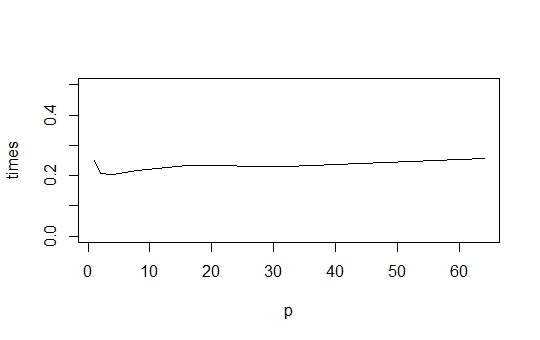
\includegraphics[width=0.6\columnwidth]{Rplot_weak_scaling} % Example image
	\caption{Weak scaling case: execution time vs number of processors $N= 10^7$}
\end{figure}
We see that the execution time is almost constant,which is what we expect with a weak scalable program.
%----------------------------------------------------------------------------------------
\section{Section 3}
Here we have the two c++ codes \textsc{sumNumbers\_mpi.cc} and \textsc{sumNumbers\_coll.cc}.

The two codes implement the pseudocode we wrote above, including the variations on the assignment.Both codes return the sum of N consecutive integers starting from 1 to N and both codes implement the calculation using a parallel approach. Both codes also address the case in which N is not divisible by the number of processors p. In this case the master node takes care of the summation of the integers that are left out from the slave processors.
The code \textsc{sumNumbers\_mpi.cc} uses only \textsc{MPI\_Send()} and \textsc{MPI\_Recv()}
while the code \textsc{sumNumbers\_coll.cc} uses the collective operations \textsc{MPI\_Bcast()} and \textsc{MPI\_Reduce()}. The codes where tested using as an input a file containing the number $N = 10^9$.

We collect a few particular times of the execution:

\begin{align} 
	\begin{split}
		&T_{read}= 3.38554 e-05 seconds\\
		&T_comp (N/P)= 0.355836\\
		\rightarrow &T_{comp} = 0.355836/100000000 = 3.5836e-9\\
		&T_comm=2.14577e-06
	\end{split}					
\end{align}
 We see that these values are close to the theoretical values we gave before,making them plausible.
%	EQUATION EXAMPLES
%------------------------------------------------

\section{Section 4}
Now its time to plot the execution time of the function we wrote, to test the strong scalability.

We plot for $N=10^9$

\begin{figure}[H] % [h] forces the figure to be output where it is defined in the code (it suppresses floating)
	\centering
	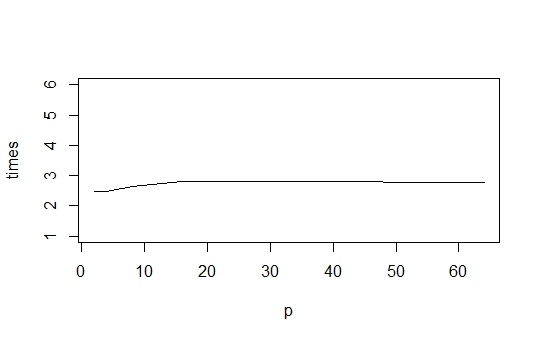
\includegraphics[width=0.6\columnwidth]{Rplot_sum_times_billion} % Example image
	\caption{execution time vs number of processors $N= 10^9$}
\end{figure}
\begin{figure}[H] % [h] forces the figure to be output where it is defined in the code (it suppresses floating)
	\centering
	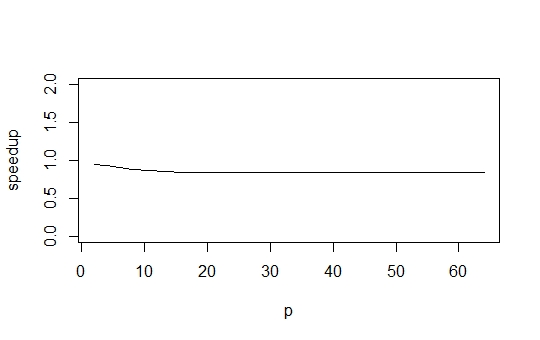
\includegraphics[width=0.6\columnwidth]{Rplot_sum_scalability_billion} % Example image
	\caption{speedup vs number of processors $N= 10^9$}
\end{figure}

\begin{figure}[H] % [h] forces the figure to be output where it is defined in the code (it suppresses floating)
	\centering
	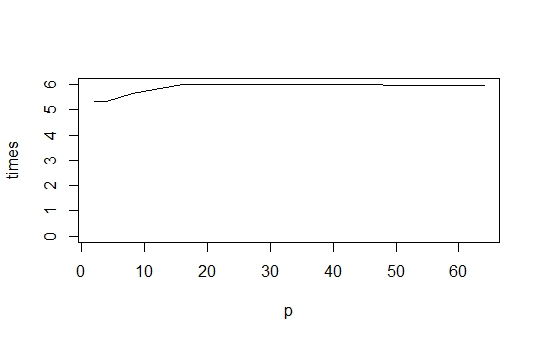
\includegraphics[width=0.6\columnwidth]{Rplot_sum_times_10billion} % Example image
	\caption{execution time vs number of processors $N= 10^{10}$}
\end{figure}
\begin{figure}[H] % [h] forces the figure to be output where it is defined in the code (it suppresses floating)
	\centering
	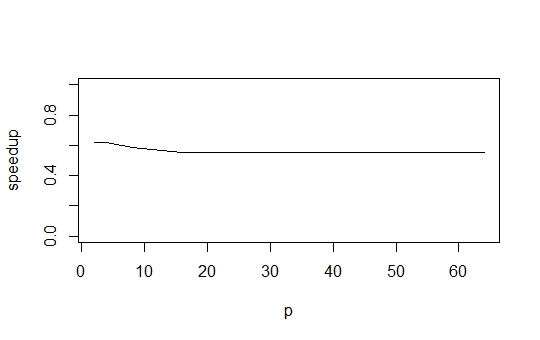
\includegraphics[width=0.6\columnwidth]{Rplot_sum_speedup_10billion} % Example image
	\caption{speedup vs number of processors $N= 10^{10}$}
\end{figure}

We see that the program isn't scaling as we predicted in our model.
Where by $10^9$ the model was perfectly scaling, our model is instead not scaling.
The exection time seems to be constant.
The executed program was the naive-implemented one,and probably the communication time increases too much and vanifies the parallelization attempt.
Basically adding more processors does not speed up to the execution time.
%----------------------------------------
\begin{figure}[H] % [h] forces the figure to be output where it is defined in the code (it suppresses floating)
	\centering
	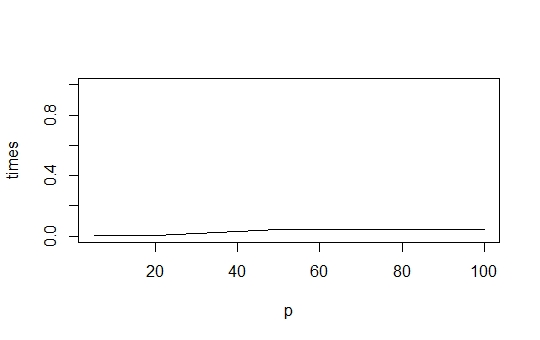
\includegraphics[width=0.6\columnwidth]{Rplot_sum_times_thousand} % Example image
	\caption{execution time vs number of processors $N= 10^3$}
\end{figure}
We get a better result if we plot the scalability for the \textit{sumNumbers\_coll.cc} code, with $N=10^{9}$. The time taken is the \textit{Walltime} given by \textit{MPI\_Walltime()}


We see that the second program scales better than the first one.
We replicated the results with $N=10^{12}$,although there is no common data type to store the result of the sum and although we couldn't test a simple serial code of the summation with such a big number,we estimate $T(1) = 5 s$.
\begin{figure}[H] % [h] forces the figure to be output where it is defined in the code (it suppresses floating)
	\centering
	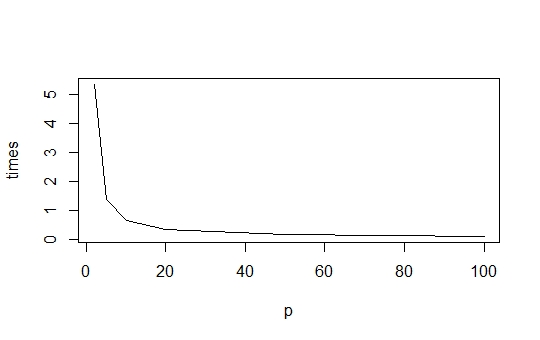
\includegraphics[width=0.6\columnwidth]{Rplot_complex_sum_times_trillion} % Example image
	\caption{execution time vs number of processors $N= 10^12$}
\end{figure}
\begin{figure}[H] % [h] forces the figure to be output where it is defined in the code (it suppresses floating)
	\centering
	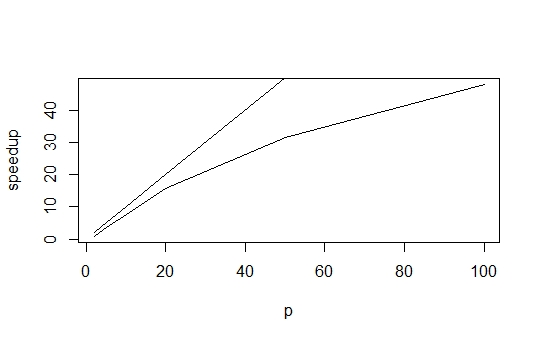
\includegraphics[width=0.6\columnwidth]{Rplot_complex_sum_speedup_trillion} % Example image
	\caption{speedup vs number of processors $N= 10^12$}
\end{figure}
%------------------------------------------------



%----------------------------------------------------------------------------------------
%	LIST EXAMPLES
%------------------------------------------------------------------------------


%----------------------------------------------------------------------------------------

%-------------------------------------------------------------

%------------------------------------------------

%----------------------------------------------------------------------------------------

\end{document}
